%%%%%%%%%%%%%%%%%%%%%%%%%%%%%%%%%%%%%%%%%%%%%%%%%%%%%%%%%%%%%%%
%%%  pts
%%%%%%%%%%%%%%%%%%%%%%%%%%%%%%%%%%%%%%%%%%%%%%%%%%%%%%%%%%%%%%%
\RequirePackage[l2tabu, orthodox]{nag}
\documentclass[onecolumn,fleqn,12pt,openany,a4paper,longbibliography,oneside]{scrbook}


\renewcommand{\baselinestretch}{1.5} 
\topmargin -1.5cm      
\oddsidemargin -0.04cm   
\evensidemargin -0.04cm  
\textwidth 16.59cm
\textheight 24cm 
\pagestyle{plain}

% special 
\usepackage{color}


% fonts
\usepackage{latexsym}
\usepackage{amsmath}
\usepackage{amssymb}
\usepackage{bm}
\usepackage{wasysym}

%by jarondl
\usepackage[font={singlespacing,footnotesize},hang]{caption}
\usepackage{subcaption}
\usepackage[numbers,sort&compress,elide]{natbib}
\usepackage{verbatim}
\usepackage{etoolbox}
  \newbool{showfigure}
  \setbool{showfigure}{true}
  
\usepackage{enumerate}
  
%%%%%%%%%%%%%%%%%%%%%%%%%%%%%%%%%%%%%%%%%%%  REMOVE FOR PRODUCTION
%\usepackage{refcheck}
% merge - {feynmann,*salam,*epr} are under one number
% elide - same as megre, but common parts appear once.
%
\usepackage{pdfpages}
% draft or final
\usepackage[nottoc]{tocbibind}
% addes the biblio to toc

%%%%%%%%%%%%%
%%% Hebrew support for hebrew abstract:
%\usepackage{ucs}
%\usepackage[utf8x]{inputenc}
%\usepackage[hebrew,english]{babel}

%\usepackage[pdfencoding=auto,colorlinks=true,pagebackref=true,pdftitle={Research Proposal}]{hyperref}
\usepackage[pdfencoding=auto,colorlinks=true,linkcolor=blue,pdftitle={Research Proposal}]{hyperref}
% doi mus be loaded after hyperref
%\usepackage{doi}
\graphicspath{{figures/}}

%%%%%%%%%%%%%%%%%%%%%%%%%%%%%%%%%%%%%%%%%%%%%%%%%%%%%%%%%%%%%%%%

% NEW 
\newcommand{\abs}[1]{\left|#1\right|}
\newcommand{\Prob}{\mbox{Prob}\,}
\newcommand{\erf}{\mbox{erf}\,}
\newcommand{\df}{{\rm d}}

% math symbols I
\newcommand{\sinc}{\mbox{sinc}}
\newcommand{\const}{\mbox{const}}
\newcommand{\trc}{\mbox{trace}}
\newcommand{\intt}{\int\!\!\!\!\int }
\newcommand{\ointt}{\int\!\!\!\!\int\!\!\!\!\!\circ\ }
\newcommand{\ar}{\mathsf r}
\newcommand{\im}{\mbox{Im}}
\newcommand{\re}{\mbox{Re}}

% math symbols II
\newcommand{\eexp}{\mbox{e}^}
\newcommand{\bra}{\left\langle}
\newcommand{\ket}{\right\rangle}

% Mass symbol
\newcommand{\mass}{\mathsf{m}} 
\newcommand{\Mass}{\mathsf{M}} 

% more math commands
\newcommand{\tbox}[1]{\mbox{\tiny #1}}
\newcommand{\bmsf}[1]{\bm{\mathsf{#1}}} 
%\newcommand{\amatrix}[1]{\matrix{#1}} 
\newcommand{\amatrix}[1]{\begin{matrix} #1 \end{matrix}} 
\newcommand{\pd}[2]{\frac{\partial #1}{\partial #2}}

% equations
\newcommand{\mylabel}[1]{\label{#1}} 
%\newcommand{\mylabel}[1]{\textcolor{blue}{[#1]}\label{#1}} 
\newcommand{\beq}{\begin{eqnarray}}
\newcommand{\eeq}{\end{eqnarray}} 
\newcommand{\be}[1]{\begin{eqnarray}\ifthenelse{#1=-1}
{\nonumber}{\ifthenelse{#1=0}{}{\mylabel{e#1}}}}
\newcommand{\ee}{\end{eqnarray}} 

% arrangement
\newcommand{\drawline}{\begin{picture}(500,1)\line(1,0){500}\end{picture}}
\newcommand{\bitem}{$\bullet$ \ \ \ }
\newcommand{\Cn}[1]{\begin{center} #1 \end{center}}
\newcommand{\mpg}[2][1.0\hsize]{\begin{minipage}[b]{#1}{#2}\end{minipage}}
\newcommand{\mpgt}[2][1.0\hsize]{\begin{minipage}[t]{#1}{#2}\end{minipage}}
\newcommand{\putgraph}[2][width=0.30\hsize]{\includegraphics[#1]{#2}}

% more
%\newcommand{\Eq}[1]{Eq.\!\!~(\ref{#1})}
%\newcommand{\Fig}[1]{Fig.\!\!~\ref{#1}}  
\newcommand{\Eq}[1]{\textcolor{blue}{Eq.\!\!~(\ref{#1})}} 
\newcommand{\Fig}[1]{\textcolor{blue}{Fig.}\!\!~\ref{#1}} 
\newcommand{\hide}[1]{}
%\newcommand{\hide}[1]{\textcolor{red}{[hidden text]}} %{}
\newcommand{\rmrk}[1]{\textcolor{red}{#1}}
%\newcommand{\Rmrk}[1]{\textcolor{blue}{\LARGE\bf #1}}

%\renewcommand{\includegraphics}[2][]{\ \\ \ FIGURE: \ \\ \ }
%\renewcommand{\cite}[1]{\textcolor{blue}{[\onlinecite{#1}}]} %{[\onlinecite{#1}]} 


%%%%%%%%%%%%%%%%%%%%%%%%%%%%%%%%%%%%%%%%%%%%%%%%%%%%%%%%%%%%%
%%%%%%%%%%%%%%%%%%%%%%%%%%%%%%%%%%%%%%%%%%%%%%%%%%%%%%%%%%%%%
\begin{document}
\frontmatter


\includepdf[pages=-]{hebstract}
\chapter*{Abstract}


We study transport and spreading in sparse disordered networks. The networks are 
constructed by assigning spatial locations to sites. Their dynamics are
described by a rate equation, with transition rates
defined both though the distance between sites as well as by a
coupling parameter. Thus, by randomizing either the locations of the sites
or the coupling parameter, we can induce disorder.



By allowing the network elements to differ by orders of magnitude,
with most of the elements vanishingly small, we create a "sparse" network.
Our interest lies in the long term transport properties of these sparse systems. 


We approach the subject of transport by looking at the spectral properties
of these networks, as well as by their resistor network analogies. We see 
that in pure $1d$ this sparsity causes subdiffusion, while in quasi $1d$ and
higher dimensions the system remains diffusive but with a reduced diffusion coefficient. 


The \emph{ERH - Effective Range Hopping -} method is suggested to estimate this diffusion 
coefficient by combining ideas from the well established \emph{VRH} scheme with 
ideas from percolation theory.


The numerical results for the diffusion coefficient are compared to the linear
estimate and to the improved \emph{ERH} result.

\newpage

{\footnotesize \tableofcontents}

\mainmatter

\part{Research Proposal}\label{part1}

\chapter{Introduction}


This proposal is about simple dynamical networks, with dynamics
that are described either by a stochastic rate equation
%
\begin{align}
  \frac{d}{dt}\mathbf{p} \quad &= \quad -\mathbf{K} \mathbf{p} \\
  \mathbf{K} \quad &\equiv \quad \textrm{diag}\{ \gamma_n \} \ \ +\ \ \textrm{offdiag}\{ -w_{nm} \} \\
  \mathbf{p} \quad &\equiv \quad \textrm{vector}\{ p_n \}
\end{align}
%
or by the Schr\"{o}dinger equation:
%
\begin{align}
  \frac{d}{dt}\psi \quad &= \quad -i \mathcal{H}\psi \\
  \mathbf{\psi} \quad &\equiv \quad \textrm{vector}\{ \psi_n \}
\end{align}
%

Regardless of the governing equation, the focus is
on disordered sparse networks, with wide distribution of energies. 
Two related aspects of these networks will be studied: their energy spectrum,
and their spreading properties. More specifically, we wish to determine
whether the networks are diffusive ($S(t)\sim t$), or sub-diffusive, and
if they are indeed diffusive, what is the diffusion coefficient. 




To simplify the discussion, we concentrate on $d$-dimensional spatial networks,
in which each node has a defined location $x_n$, and each edge has an associated 
energy barrier $\epsilon_{nm}$. The transition rates are then defined to be:
%
\begin{align}
w_{nm} \quad = \quad w_0 \eexp{-\epsilon_{nm}}B(x_n-x_m)
\end{align}
%
Where $B(r)$ describes the dependence of the coupling on the
distance between sites.


The model we start with has its sites distributed randomly and uniformly throughout
a $d$-dimensional hypercube, with $B(r) = \exp(-r/\xi)$. The disorder is defined by the location
of the sites, and its effect on the connectivity of the network can be manipulated through the 
parameter $\xi$. 



%%%%%%%%%%%%%%%%%%%%%%%%%%%%%%%%%%%%
\section{Matrices of interest}\label{sec:matrix_categories}







This work concern {\rm real} matrices that describe {\em disordered} 
one- two- and quasi-one- dimensional structures. Such matrices 
are of physical interest in various applications including:

\begin{enumerate}[A. ]
\item Resistor networks / random walk / hopping 
\item Rate equations / relaxation processes 
\item Mechanical elastic vibrations ("balls and springs")
\item Electrical R-L-C circuits
\item Hermitian quantum dynamics with time-reversal symmetry. 
\item Non-Hermitian quantum dynamics with any anti-unitary symmetry. 
\end{enumerate}

In particular we note that the Mott impurity hopping problem 
belongs to category A. The problem of Sinai spreading ("random 
walk in random environment") belongs to category B. 
The theory of heat conduction belongs to category C. 
Studies of wave-packet dynamics belong to E, and 
in particular the recent interest in systems that are described by 
a non-Hermitian PT symmetric hamiltonian belongs to category F.

In the present proposal we would like to emphasize the 
implications of {\em sparsity}, meaning extreme disorder 
due to log-wide distribution of matrix elements. 
We note that {\em localization} and {\em percolation} are strongly 
related aspects in the analysis of transport in such systems. 


The real matrices that we consider can be characterized 
by several properties, which we list here in order of increasing 
complexity, and further elaborate below:

\begin{enumerate}
\item Symmetry.
\item Non-negativity.
\item Conservation.
\item Detailed balance.
\item Frustration.
\item Diagonal disorder.
\item Broken reality.
\end{enumerate}

The eignevalues of a real matrix are the roots of a characteristic 
polynomial that has real coefficients. Hence the spectrum consists 
of real eigenvalues, and optionally also pair of complex-conjugate 
values. 

By "non-negativity" we mean that all eigenvalues are real and 
non-negative: for example in the context of rate equations it means 
that all the eigen-modes are decaying except the steady state 
that has zero eigenvalue. 

By "Broken-reality: we mean that some of the eigenvalues  
become complex: in particular this might happen 
as we vary some control parameter. The studies of "PT broken symmetry" 
provides an example for such scenario. One should realize that  
a complex eigen-state that is associated with a complex eigenvalue 
has a {\em lower} symmetry than that of the Hamiltonian.

It is most common to consider a {\em symmetric} matrix. 
All the eigenvalues of such matrix are real. 
Such matrices appear in Hamiltonian dynamics 
if the system has anti-unitary (say time reversal) symmetry.  

A special sub-class of symmetric matrices consists of those 
that are both non-negative and conserving. Such matrices
can be regarded as describing a "resistor network".
They have positive off-diagonal elements that describes 
the connectors, while their diagonal elements are determined 
such that the probability (or the charge) is conserved. Namely 

%gamma_n \equiv ... = ... 
%
\begin{align}\label{eq:zero_sum}
\gamma_n \equiv -\sum_{m\ne n} w_{mn}
\end{align}
%

The eigenvalues of a non-negative conserving symmetric matrix, 
are all non-negative and represent decay or diffusion modes of the network. 
Only the ergodic state is non-decaying with zero eigenvalue.   

More generally rate-equation matrices are non-negative, conserving, 
but non-symmetric. Hence they have real positive eigenvalues 
that are associated with the decay modes of the system, 
and a zero mode that describes the steady state.  

It should be realized that the dynamics that is generated 
by  a "resistor network" matrix ("infinite temperature") 
resembles diffusion or percolation process, while that of 
a ``finite temperature" network (non-symmetric matrix) has to 
do with Sinai spreading (as discussed in \autoref{sec:anderson}).  

A special sub-class of conserving non-negative matrices 
are {\em detailed-balanced}. See \autoref{sec:detailed_balance} for precise definition. 
Hence there is a simple "canonical" expression for their 
ground state. More generally the system might be frustrated 
hence the "non-equilibrium" steady state might carry current.

The matrix that describes a system that is composed 
of balls connected by springs is similar to that of a 
rate equation, but has diagonal elements that might contain 
an additional contribution that reflects a pinning potential 
that attaches each ball to a fixed location.   


%%%%%%%%%%%%%%%%%%%%%%%%%%%%%%%%%%%%%%%%%%%%%%%%%%%%%
%\section{TODO VRH}

%%%%%%%%%%%%%%%%%%%%%%%%%%%%%%%%%%%%%%%%%%%%
\section{Motivations for the model}
%% bullets - where does this model appear - balls and springs (leads to heat) - capacitors
%%             - conductance hopping

We have kept the model abstract and general on purpose, so that it
might fit a large number of physical situations. Some physical applications include:
%
\begin{itemize}
  \item
    Balls and Springs\ - \ A simple mechanical system of balls connected to each
      other by springs. The vibrational modes of the system are phonons, which conduct heat.
  \item
    Capacitors and Resistors\ -\ An electrical network of capacitors connected to each other
      by resistors.
  \item 
    Mott impurity hopping\ - \ This kind of conductance arises from hopping 
      between impurities.
\end{itemize}


%%%%%%%%%%%%%%%%%%%%%%%%%%%%%%%%%%%%%%%%%%%%%%%%%%%%%%%
\section{The Anderson localization}\label{sec:anderson}

In the Anderson model\cite{anderson_absence_1958}, a nearest neighbor network is formed
on a lattice. The bonds are all equal, and the on-site energies are random.
For $d=1$ and $d=2$, all states are localized, while for $d>2$, there exists
a transition between localized and extended modes. The common knowledge
is that every uncorrelated disorder causes localization. However, if the system
has an ergodic mode, i.e.\ every site has the same occupancy, then the localization length 
diverges, practically meaning effective delocalization. Moreover, if the energy
of this mode sits on the lower edge of the spectrum, this effective delocalization 
causes regular diffusion.


%The expressions for \emph{dc} conductivity and average conductance 
%\cite{kubo_statistical-mechanical_1957,greenwood,thouless_electrons_1974,braun_level_1997}
% can be written as
%
%\begin{align}
%\sigma &= \frac{\pi e^2}{m^2 V} \sum_{\alpha,\beta} 
%                 \left|\bra\alpha |\hat{p}|\beta\ket\right|^2 \delta(E_F-E_\alpha)\delta(E_F-E_\beta) \\
%\langle G \rangle &= \langle \sigma \rangle L^{d-2}
%\end{align}
%



There are several routines used to distinguish between exponentially localized and delocalized modes.
The most straight forward one seems to be the participation number (PN) 
\cite{edwards_numerical_1972}, which is defined by its inverse:
%
\begin{align}
PN^{-1} \ =\ \sum_i p_i^2
\end{align}
where $p_i$ is the probability to be in a specific site, equal to $|\psi_i|^2$ 
for a quantum wave function. For a fully extended mode $PN\sim N$, while for a state
occupying only one site $PN = 1 $.


Another idea called Thouless curvature or Thouless conductance 
\cite{edwards_numerical_1972,thouless_electrons_1974,braun_level_1997}, is based
on the idea that localized eigenmodes are almost not sensitive to boundary conditions. We apply a 
phase change $\phi$ across the boundary, (due to gauge invariance the specific spot is irrelevant),
and check the resulting change in the eigenvalues. 
In an ordered system with extended modes, $\phi=\pi$ will cause an energy
shift larger than the level spacing. 
Using perturbation theory on Kubo's equation \cite{kubo_statistical-mechanical_1957},
Thouless defined a conductance that is proportional to the diffusion: 
\begin{align}\label{eq:thouless}
\bra g_T\ket  \equiv \pi \frac{\bra \left|\left. \frac{\partial ^2 E^{(n)}}{\partial \phi^2}\right|_{\phi\rightarrow 0}\right|\ket}{\Delta}
\end{align}
where $\Delta$ is the level spacing.



Because we have defined the diagonal by requiring each row and column to nullify,
there always exists a special extended $\lambda=0$ mode with all probabilities equal. 
Actually, in our $d\le 2$ models, the localization length diverges as $\lambda\rightarrow 0$,
So that while the states are localized by definition, in practice they may be very wide
compared to the system length.



%%%%%%%%%%%%%%%%%%%%%%%%%%%%%%%%%%%%%%%%%%%%
\section{Modeling quantum diffusion with resistor networks}

%In past work \cite{cohen_wave_2000} 

In a model described by a Hamiltonian 
%
\begin{align}
\mathcal{H} = \textrm{diag}{E_n} + \epsilon {V_{nm}}
\end{align}
%
according to the first step of perturbation theory,
for very short time the transition probability is:
%
\begin{align}
 p(n, n_0)\ =\ \left| \epsilon \bra n| V |n_0\ket t\right|^2 \ = \ \epsilon^2 t^2\left| \bra n| V |n_0\ket \right|^2
\end{align}
%
This suggests that for some short time scale, the ballistic behavior
of the system might relate to the conductivity of the rate equation $G_{nm} = \left| \bra n| V |n_0\ket \right|^2$.




%%%%%%%%%%%%%%%%%%%%%%%%%%%%%%%%%%%%%%%%%%%%%%%
\section{Heat conductance}

One can take one of our suggested models, and couple each end to a different heat bath.
The total heat conductance of the sample is defined by:
\begin{align}
J = \int_0^\infty \rho(\lambda) g(\lambda) d\lambda
\end{align}
where $\rho(\omega)$ is the density of states, and $g(\lambda)$ is 
a transmission coefficient for a phonon at energy $\lambda$.
 
However, many one-dimensional models 
\cite{narayan_anomalous_2002,dhar_heat_2001,lepri_anomalous_1998,savin_heat_2002} 
exhibit sample size scaling of the form
%
\begin{align}
g(\lambda)    &\propto L^\alpha
\end{align}

It is debated whether for $d=1$ systems
with momentum conservation,  $\alpha=1/3$,$\alpha=2/5$ or neither
\cite{narayan_anomalous_2002,delfini_comment_2008,dhar_dhar_2008,wang_power-law_2011}.
For several systems it has been shown that $\alpha$ depends on some tunable potential \cite{tong_wave_1999},
and it also depends on the spectrum of the baths \cite{dhar_heat_2001}.



$g(\lambda)$ is highly affected by the localization length of this mode, 
and one way to find it is via Thouless' curvature \autoref{eq:thouless}.
The high frequency eigenmodes are strongly localized, hence only the
first part of the spectrum contributes to the heat flux. Based on this idea,
the heat flux can be estimated \cite{lepri_thermal_2001,bodyfelt_unpub},
by the number of wide modes.



%%%%%%%%%%%%%%%%%%%%%%%%%%%%%%%%%%%%%%%%%%%%%%%%%%%%%
\begin{comment}
\section{Banded matrices spectrum}


For wide bandwidth and uncorrelated matrix elements, the high eigenvalues
should follow the Wigner semicircle law ($g(\lambda) = \frac{2}{\pi R^2}\sqrt{R^2-\lambda^2}$)
\cite{erdos_local_2012,fyodorov_scaling_1991,wigner_characteristic_1955}. However,
the low eigenvalues can still follow other rules, allowing for a transition
between diffusion and subdiffusion.
\end{comment}




%%%%%%%%%%%%%%%%%%%%%%%%%%%%%%%%%%%%%%%%%%%%%%%%%%%%%%
%\section{Sinai diffusion}




%For example, by adding spatial correlations, the behavior can be changed 
%from $S(t) \sim (\log t)^4$ to $S(t) \sim (\log t)^y$ with $y \in [4,\inf]$ \cite{stanley_generalisation_1987}.

%%%%%%%%%%%%%%%%%%%%%%%%%%%%%%%%%%%%%%%%%%%%%%%%%%%%%%%
%\section{Organization}

%The organization of this proposal is in parts.
%\autoref{part1} includes this introduction,
%the objectives of the proposal and further background. 
%In \autoref{part2} we present the work accomplished so far.
%In \autoref{part3} lies the appendix, including some derivations,
%and an article accepted for publication at PRE, available in the arXiv \cite{de_leeuw_diffusion_2012}.

\chapter{Objectives}



%%%%%%%%%
\section{Diffusion or Subdiffusion in $2d$}

For the stochastic random network, the question of diffusion in most $1d$ systems was analytically solved in \cite{alexander_excitation_1981}. 
The $2d$ case is, as far as we know, not yet analytically solved, and is much less clear. 
In \cite{amir_localization_2010} it is claimed that in low density systems subdiffusion of
order $\sim log^d$ should occur. We wish to examine these networks through their spectral
properties to find out if this is indeed the case. Our focus will be on low densities,
and on checking whether there exists a transition between low densities and high densities.


%%%%%%%%%
\section{Geometrical implications}

The aforementioned density changes are equivalent to rescaling of the system size,
while keeping the site locations in place, meaning that the geometry of the problem 
does not change. But does the geometry matter at all? Of course, the geometric properties
of the system are reflected in the statistics of the distances,
and by extension in the statistics of the transition rates. 
However, there is more information in the $W_{nm}$ matrix than just the statistics of its elements.
The question arises: Are the statistics all that is needed to understand the physics of the system? 
We shall check numerically if a randomized matrix with the same statistics behaves the same.



%%%%%%%%%
\section{Banded sparse matrices}

Between the $1d$ nearest neighbor network and the $2d$ network,
lie the quasi $1d$ network, which allows transitions to further neighbors.
The conductance of quasi-$1d$ banded sparse matrices was studied numerically in \cite{stotland_random-matrix_2010}. There, they use \emph{Variable-Range-Hopping} in the sparse regime, where 
$(\text{sparsity}\cdot \text{bandwidth}) \ll 1$. 
However, in this work it is not clear what are the limits on either sparsity or bandwidth, and in particular where is the cross between the validity regime of VRH and that of SLRT. We will try to understand this issue analytically.


% TODO A specific version of these matrices were also studied in \cite{janssen_correlated_2000}.

%%%%%%%%%%%
\section{Assymetric VRH}

In the networks we have discussed so far, each site had the same potential. Once
we allow different potentials, the site occupation probabilities change.
This can be accommodated for by modifying the transition rates by Boltzmann's factor. This is called \emph{VRH- Variable Range Hopping}\cite{ambegaokar_hopping_1971}, and has been widely studied. 
Derived from Fermi statistics, it is shown that it is equally likely to go up in energy as it is to go down in energy.
Therefore, the common practice is to treat the system as a symmetric resistor network,
but we want to ask if there are cases where this reduction to a symmetrical network is not valid.
If such cases exist we wish to develop a better estimation method for the transport. 


% stotland Errata variable activation energy.. 
%%%%%%%%%
%\section{stotland's errata model}




% Could maybe add here an additional item from the notes if necessary.

%%%%%%%%%
\section{The spectral properties of Sinai diffusion in $1d$}

In a symmetric $1d$ random rate system, there is regular diffusion if the harmonic average is bounded, i.e.\ if
%
\begin{align}
 \sum_n \frac{1}{w_n} < \infty 
\end{align}
%

On the other hand, for an asymmetric system, an activation energy builds up, and a Sinai diffusion behavior is followed.
The conductance is exponentially small in the length, and the spreading is anomalous. The difference between those two models is clearly highly significant. We wish to investigate the difference between the models,
and the relation of this difference to the spectral properties of the model.

%%%%%%%%%
\section{Sinai diffusion in $2d$}

We shall inspect the spectral properties, and spreading behavior of a $2d$ asymmetric system. The
$2d$ case is much different than the $1d$ case, because particles can circumvent barriers. Interestingly,
a nearest neighbor lattice can be constructed to present the same long time spreading as the $1d$ lattice \cite{blumberg_selinger_diffusion_1989}.
The question is whether having nearest neighbor links only is a necessary condition for this behavior,
and how does this relate to the spectral properties of the $2d$ system.


%%%%%%%%%
\section{The charge carrier discreteness}\label{sec:discreteness}

Our work so far considered probability rate equations, which are valid for a single particle in the network.
Having many non interacting particles is equivalent to having many realizations of a single particle,
leaving the picture intact. However, if we have multiple \emph{interacting} particles in the network, additional factors may contribute. For example,
a single occupancy rule (i.e.\ each site may have up to one particle) may cause Fermi blocking. Another
issue is that the single particle behavior might be sub-diffusive while the bulk spreading is diffusive \cite{richards_theory_1977,hung_diffusion_2012}.


%%%%%%%%%%
\section{Generalization to a quantum state}

Up to now, we have concentrated on Markovian networks, dealing with the probabilities without phases.
We will try to generalize the work to solve Hamiltonian matrices of the same genre.
With a coherent Hamiltonian, 
we expect suppression of the diffusion due to Anderson localization. However, finite
dephasing time in this system will lead to noticeable transient diffusion.
We intend to examine the applicability of the resistor network picture for 
the calculation of the diffusion coefficient in these quantum networks, beginning with
a simple model described by a real symmetric Hamiltonian:
%
\begin{align}
  \mathcal{H}_{nm} = \textrm{random}[\pm] \eexp{-\textrm{random}[x]} \qquad 0<|n-m|\le b
\end{align}
%
Where the parameter $x$ is distributed uniformly $x\in [0,\sigma]$. 

% (1d and 2d) are different sections.

% 1d . Having a site, with random rates, we have diffusion - harmonic average (less or equal to inf).
%      Now, if the rates are assymetric, we have sinai diffusion (Daniel).
%      The conductance is exponentially small in the length, which is very different from before.
%      The spreading is anomalic. 
%      (Refs. in Daniel's paper. Assymetric random work.) Activation potential in stochastic field.
%      It is a general claim that an activation potential will be created for any random selection.
%      WHAT is the relation between Sinai's work and spectral properties? What about the temporal dependance.
%% This is important. Derrida doesn't have a solution. Write a page about the amazing difference between those
% two models, and relate to spectral properties.
%  Google : Sinai diffusion 2D.


% Read Halperin and Begouker. Mott -> resistor network. Fermi energy - statistics - The asymmetry disappears (It is equally 
% likely to go "up" as it is to go "down" in energy.
% Amir wrote about it. Also in textbooks.

% The charge carrier discreteness.
% The rate equation is for one body - probability.
% If there are 100 particles with no interaction - that's the same.
% What about blocking due to other particles (For example Fermi's exclusion). 
% "Mean field" - using averages. Fermi Blocking. Eq 64 in stotland's X section.


% Kottos. Quantum version. Localization etc. 


\part{Completed Work and Preliminary Analysis}\label{part2}
\chapter{Completed Work}


This work was published at Physical Review E \cite{de_leeuw_diffusion_2012},
and reprinted here in \autoref{sec:papers}. In the
following sections we will provide an overview
of the main results.


%%%%%%%%%%%%%%   Overview over article should not include too much equations
%%  bottom line - take home message - the derivations should ref the article

%%  
%%  remove the techinalities - 
%%     using the procedure we have calculated for.. blah blah
%%       see figure. (leave plots only if neccessary to buttom line).
%%
%%  geometry plots - maybe try with normal scale.
%%                   if that doesn't work, leave the figure out.



%%%%%%%%%%%%%%%%%%%%%%%%%

%%%%%%%%%%%%%
%\section{Article abstract}
%\rmrk{This is the article abstract..}


We have studied random networks whose dynamics are
described by a rate equation, with transition rates $w_{nm}$
that form a symmetric matrix (\autoref{sec:matrices}),
with a diagonal conforming to \autoref{eq:zero_sum}. 
%
The long time evolution
of the system is characterized by a diffusion coefficient~$D$.
In one dimension it is well known that $D$ can display an abrupt
percolation-like transition from diffusion (${D>0}$)
to sub-diffusion (${D=0}$). 
%
A question arises whether
such a transition happens in higher dimensions.
Numerically $D$ can be evaluated using a resistor network
calculation, or optionally it can be deduced from 
the spectral properties of the system. Contrary to a recent 
expectation that is based on a renormalization-group analysis, 
we deduce that $D$ is finite.
%
We suggest an ``effective-range-hopping'' procedure to evaluate $D$,
and contrast the results with the linear estimate.
The same approach is useful for the analysis of 
networks that are described by quasi-one-dimensional  
sparse banded matrices. 


%%%%%%%%%%%%%%%%%%%%%%%%%
\section{The effective range hopping procedure}


The basic idea behind \emph{ERH} (effective range hopping) is that in the linear
expression, nearby sites 
with $r\ll 1$ (and therefore $w \gg 1$ ) are over represented in
the diffusion coefficient calculation. While the transition to
these sites is indeed high, the distance covered is not enough
to form a percolating cluster. Therefore, we use a threshold based
on percolation theory and flat-down the rates higher then this threshold.
This produces a smooth crossover between the linear
estimate and the \emph{VRH} estimate.


Using the \emph{ERH} procedure we have calculated the diffusion for several models.


For the degenerate hopping model we obtained:

\begin{align}
D_{\tbox{ERH}} &=  \mathrm{EXP}_{d{+}2}\left(\frac{1}{s_c}\right)  \  \eexp{-1/s_c}  \ D_{\tbox{linear}}
\end{align}
%
For infinite dimensions ($d\rightarrow\infty$),  we have $\mathrm{EXP}_{d{+}2}\  \eexp{-1/s_c} = 1$. 
This means that the ERH expression converges with the linear expression.
For low dimensionality, the exponent dominant.


For the Mott Hopping model,
%
\begin{align}
D_{\tbox{ERH}} &=\mathrm{EXP}_{d{+}3}\left(\epsilon_c\right)  \  \eexp{-\epsilon_c}  \ D_{\tbox{linear}}
\end{align}
%


For the flat-profile banded $1d$ model,
\begin{align}
D_{\text{ERH}} \ \ &= \ \ 
\ \frac{1}{\sigma}\left[ 
\left(1+\frac{n_c}{2b}\sigma\right)\eexp{-\frac{n_c}{2b}\sigma} - \eexp{-2\sigma}
\right] \ \tilde{b} w_0 \\ &=\ \ 
\ \frac{\left(1+\frac{n_c}{2b}\sigma\right)\eexp{-\frac{n_c}{2b}\sigma} - \eexp{-2\sigma}}
       {1 - \eexp{-2\sigma}}
   \ D_{\tbox{linear}}
\end{align}



%%%%%%%%%%%%%%%%%%%%%%%%%%%%%%%%%%%%%%%%%%%%%%%%%%%%
%%%%%%%%%%%%%%%%%%%%%%%%%%%%%%%%%%%%%%%%%%%%%%%%%%%%
\chapter{Preliminary analysis}



%%%%%%%%%%%%%%%%%%%%%%%%%%%%%%%%%%%%%%%%%%%%%%%%%%%
%%%%   PTA                                    %%%%%
%%%%%%%%%%%%%%%%%%%%%%%%%%%%%%%%%%%%%%%%%%%%%%%%%%%
\section{Heat transport in sparse banded Hamiltonians}\label{sec:PTA}


We have analyzed a model of springs and masses described in \autoref{sec:app_heat}.
The Hamiltonian is quadratic in the $K$ matrix as defined in \autoref{eq:K_matrix},
which means that the eigenvalues $\lambda$ of $K$ determine the frequencies $\omega^2 = \lambda$.
The eigenmodes are of course the same. The analysis of this model in the resistor network perspective
and the lower-eigenvalues spectral analysis perspective is presented in the article, and we now
turn to inspect the heat transport angle.


As explained earlier, in contrast to the low-eigenvalue-only DC conductance, 
the total heat conductance is defined by the
sum over the heat conductances of the participating modes:
%
\begin{align}
G \ =\ \sum_n g(\lambda_n)
\end{align}
%
It is common to assume
that the temperature of the baths is high enough for all the modes to
participate, and for the bath spectrum to be white, meaning that all frequencies
have the same weight. The heat conductance of an eigenmode can be calculated
using the Landauer or the Kubo formalism, or, alternatively, can be estimated
via the PN (participation number), or the Thouless curvature. 
In recent studies \cite{bodyfelt_unpub} of \emph{pinned}\cite{roy_role_2008} banded matrices,
two groups of PN values were observed, and by counting the number of modes in the
higher PN group, the total conductance scaling was found. 



In \autoref{fig:pta} we have extended this analysis by studying the
effects of pinning, and by introducing sparsity. Also, we have
numerically calculated the Thouless conductance,
which we expect to correlate with $PN$. Disregarding major numerical issues,
the correlation seems to hold, see \autoref{fig:PN_g_scatter}.


As presented in \autoref{sec:heat}, the thermal conductance depends
on all the wide modes. The DC conductance, on the other hand,
depends on the $\lambda\rightarrow 0$ modes only. It seems that
for sparse systems these definitions coincide, since only 
the $\lambda\rightarrow 0$ modes are wide.


%%%%%%%%%%%%%%%%%%%%%%%%%%%%%%%%%%%%%%%%%%%%%%%%%%%%%%%%%%%%%%%%%%%%%%%%%%%%
%%  The following figure is displayed on rp.pdf but not on pta_dts_as_notes
%%     Because of the boolean showfigure.
%%%%%%%%%%%%%%%%%%%%%%%%%%%%%%%%%%%%%%%%%%%%%%%%%%%%%%%%%%%%%%%%%%%%%%%%%%%
\notbool{showfigure}{\begin{comment}}{}

\begin{figure}[H]
  %\subfloat[Low sparsity]{
  \begin{subfigure}{.45\linewidth}\centering
    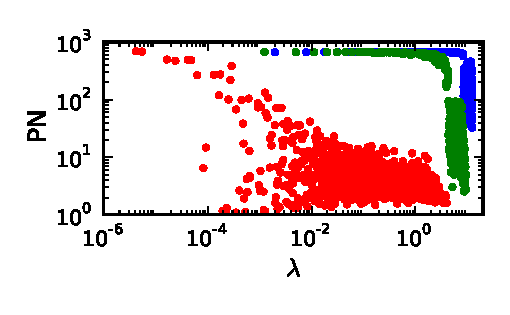
\includegraphics[width=0.99\linewidth]{pta_nopin}
    \caption{}\label{fig:PN_kottos_nopin}
  \end{subfigure}
  %
  \begin{subfigure}{.45\linewidth}\centering
     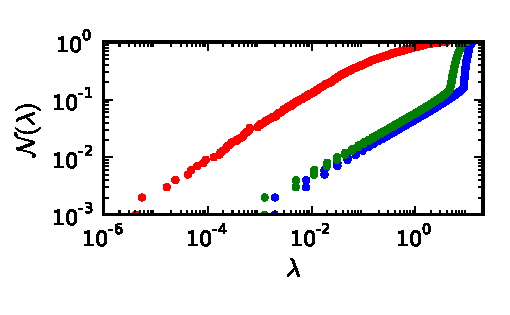
\includegraphics[width=0.99\linewidth]{pta_ev_nopin}
  \caption{}\label{fig:ev_dist}
  \end{subfigure}\\ % end of row
  %
 % \caption{}
 % \end{figure}
 % \begin{figure}[H]
  %
    \begin{subfigure}{.45\linewidth}\centering
    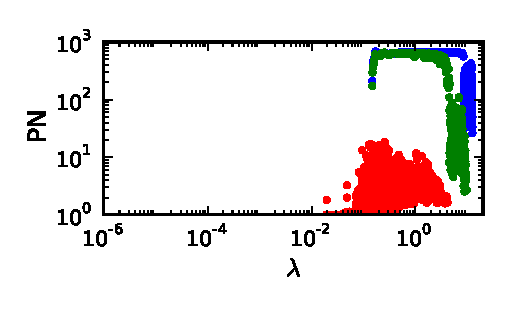
\includegraphics[width=0.99\linewidth]{pta_pin}
    \caption{}\label{fig:PN_kottos_pinning}
  \end{subfigure}     
  %
  \begin{subfigure}{.45\linewidth}\centering
     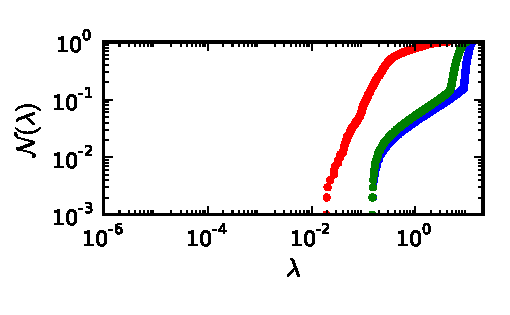
\includegraphics[width=0.99\linewidth]{pta_ev_pin}
  \caption{}\label{fig:ev_dist_pin}
  \end{subfigure}
    \begin{subfigure}{.45\linewidth}\centering
    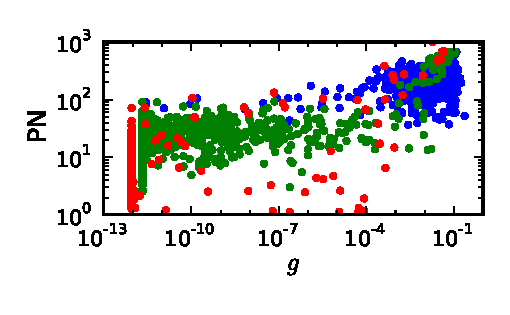
\includegraphics{pta_scatter_g}
  \caption{}\label{fig:PN_g_scatter}
  \end{subfigure}
  \caption{For all the plots $N=1000$ and $b=5$. 
           In blue $\sigma=0.1$, green $\sigma=0.6$ and red $\sigma=10$, where higher
           $\sigma$ means more sparsity.
           %%%%
           In (\subref{fig:PN_kottos_nopin}) with low $\sigma$ (blue) we see two groups of PN values.
           This distinction is lost for higher $\sigma$ (red).
           %%
           In (\subref{fig:ev_dist}) we plot the cumulative distribution of
           the eigenvalues, presenting clear diffusive behavior, for any $\sigma$.
           %%%%%% pinning
           In (\subref{fig:PN_kottos_pinning}) and (\subref{fig:ev_dist})
           we see the effects of diagonal disorder (pinning)
           on the spectrum. We see clearly that the lowest eigenvalues 
           are affected, and their corresponding PN is much lower. The spectrum
           reveals sub-diffusive behavior.
           %%%g 
           In (\subref{fig:PN_g_scatter}) we compare the Thouless conductance
           $g$ with the participation number. 
           The presented points do seem to be correlated, but due to numerical issues,
           many values of $g$ are below the precision limit (seen as a vertical line in the plot), 
           up to $936$ from $1000$ for $\sigma=10$. 
  }\label{fig:pta}
\end{figure}

\notbool{showfigure}{\end{comment}}{}




%%%%%%%%%%%%%%%%%%%%%%%%%%%%%%%%%%%%%%%%%%%%%%%%%%%%%%%%%
%%%%%%%%%   DTS
%%%%%%%%%%%%%%%%%%%%%%%%%%%%%%%%%%%%%%%%%%%%%%%%%%%%%%%%%

%%%%%%%%%%%%%%%%%%%%%%%%%%%%%
\section{Quantum spreading in a sparse banded Hamiltonian}\label{sec:dts}

In this section the numerical work was done by our collaborators,
Eli Halperin and Tsampikos Kottos of Wesleyan university.


We define a Hamiltonian
\begin{align}
\mathcal{H}\ \ &=\ \ \epsilon B_{nm}\\
B_{nm} \ \ &= \ \ \textrm{random}[\pm]\eexp{-x}\qquad 0<|n-m| \le b \\
x \ \ &= \ \ \textrm{random} \ \in [0,\sigma]
\end{align}
that depends on three parameters, $\epsilon$, $b$ and $\sigma$. The $\sigma$
parameter controls the sparsity, and $b$ is the bandwidth, and $\epsilon$
defines the units of frequency.
In past works \cite{cohen_wave_2000,stotland_random-matrix_2010} it was deduced that the diffusion coefficient 
in a disordered banded system can be calculated as:
\begin{align}
D_0 \ \ &=\ \ \left[b\ \textrm{Var}[B_{nm}]\right]^{1/2}\ b^2\epsilon \\
\textrm{VAR}(B_{nm}) \ \ &=\ \ \int_0^\sigma \left(\pm \eexp{-x}\right)^2 \frac{dx}{\sigma}\ \ 
 =\ \  \frac{1-\eexp{-2\sigma}}{2\sigma} \\
 D_0\ \ &\propto\ \ b^{2.5}\ \sqrt{\frac{1-\eexp{-2\sigma}}{2\sigma}} 
\end{align}

To question the validity of this result in the case of high sparsity,
we plot in \autoref{fig:D_of_s} the numerical results for $D$ divided by 
the speculated $D_0$. The results reveal that the sparsity affects the diffusion coefficient.
We see that as the system becomes more sparse, the diffusion coefficient is suppressed,
and as might be expected, the lower bandwidth ensembles are more
susceptible, as the system is more vulnerable to disconnections.


The next speculation is to use the suppression factor for sparse networks 
obtained in our previous work \autoref{sec:papers}:
%
\begin{align}
g_s(\sigma, b)\ \ &=\ \ \frac{D_{ERH}}{D_{\textrm{linear}}}\ \ =\ \ 
\frac{  \left(1+\frac{n_c}{b}\sigma\right)\eexp{-\frac{n_c}{b}\sigma}
                                              - \eexp{-4\sigma}}{1-\eexp{-4\sigma}}\\
\textrm{With } n_c\ &\approx 2
\end{align}

In \autoref{fig:d_vs_g} we plot a log-log scale, assuming a relation:
%
\begin{align}
\frac{D}{D_0}\ \ \approx \ \ C\ \ g_s(\sigma,b)^\gamma
\end{align}

From numerical fitting we see that $C\approx \frac{3}{4}$, 
and $\gamma$ is difficult to extract from this data set. We assume
that a wider range of $\sigma$ values will offer more knowledge.

\begin{figure}
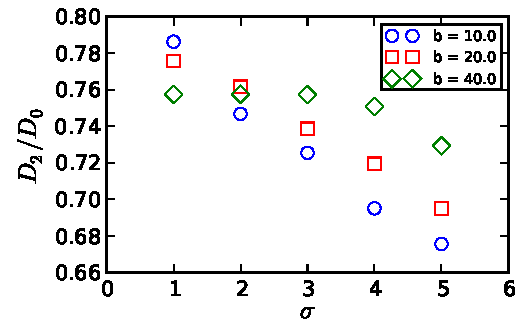
\includegraphics{dts_D2}
\caption{The transient diffusion coefficient for quantum spreading in
a banded sparse network. The ratio $D/D_0$ between the numerical diffusion 
coefficient and the expected value decreases as $\sigma$ increases. The effect
is stronger for low bandwidth.}\label{fig:D_of_s}
\end{figure}


\begin{figure}
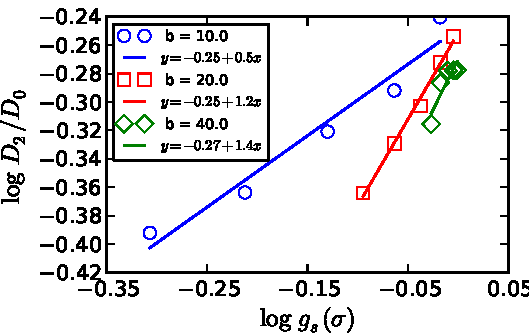
\includegraphics{dts_D2_vs_gs_loglog}
\caption{Scaled $D$ vs $g_s$. }\label{fig:d_vs_g}
\end{figure}


%\part{Preliminary Analysis}


\part{Appendix}\label{part3}
\appendix

\chapter{Published Paper}\label{sec:papers}

\includepdf[pages=-]{PhysRevE_86_051120}
%%%%%%%%%%%%%%%%%%%%%%%%%%%%%%%%%%%%%%%%%%%%%%
%%%%%%%%%%%%%%%%%%%%%%%%%%%%%%%%%%%%%%%%%%%%%%
\chapter{Spacing Statistics in $d$-dimensions}\label{sec:spacing}

Some clarifing points regarding the statistics of uniformly distributed sites 
will be made in this section.


There are $N$ sites distributed randomly within a $d$-dimensional
hypercube of volume $L^d$. We define a typical length $r_0$ by:
%
\begin{align}
\frac{L^d}{r_0^d} \ =\ N
\end{align}
%
From now on we shall ignore boundary conditions, assuming $N$ is large enough.
In the numerics we have used periodic boundary conditions.


If we choose some arbitrary point as the origin, the distribution of sites
around this point will be:
%
\begin{align}\label{eq:rho}
\rho(r)dr = \frac{\Omega_d r^{d-1}}{r_0^d}dr
\end{align}
% 
Where $\Omega_d$ is the $d$ dimensional solid angle:
%
\begin{align}
\Omega_d \ =\ 2,\ 2\pi,\ 4\pi, \ldots
\end{align}
%

The distribution of the nearest neighbor distance can be 
derived \cite{hertz_uber_1909,*Chandrasekhar_stochastic_1943,*Torquato_nearest-neighbor_1990},
using a differential equation. 


Let us denote by $P(r)$ the probability that the first near neighbor will be
between $r$ and $r+dr$. The probability of having no neighbors up to distance $r$ is
%
\begin{align}
P_0(r) \ =\  1 - \int_0^r P(r)dr
\end{align}
$P(r)$ must equal the probability of having no neighbors up to distance $r$ times
the probabilty of finding a neighbor between $r$ and $r+dr$. So $P(r)$ must satisfy:
%
\begin{align}
P(r) \ &=\ P_0(r) \times \rho(r) \ =\ \left[ 1-\int_0^r P(r)dr \right] \rho(r) \\
\frac{P(r)}{\rho(r)}\ &=\  1-\int_0^r P(r)dr \\
\frac{d}{dr}\left(\frac{P(r)}{\rho(r)}\right) \ &=\ -\rho(r)\frac{ P(r)}{\rho(r)}
\end{align}
%
Which has the solution:
%
\begin{align}
P(r) \ &=\ \rho(r) \eexp{-\int_0^r \rho(r) dr} \\
       &=\ \frac{\Omega_d r^{d-1}}{r_0^d} \eexp{-\frac{\Omega_d}{d} \left(\frac{r}{r_0}\right)^d}  \label{eq:spacing_dist}
\end{align}
%
Where in the last step we have plugged in $\rho(r)$ from \autoref{eq:rho}
%


%The probability to have an empty surface of radius $r$ and thickness $\Delta r$
%surrounding the origin is 
%
%\begin{align}
%P_0(r<x<r+\Delta r) = (1-\rho(r)\Delta r)
%\end{align}
%
%To have an empty hypersphere, we need to have all of the surfaces empty. 
%So we can formally write $r=N\Delta r$, and multiply the probabilities:
%
%\begin{align}
%P_0(r) = \lim_{N\to \infty} \left( 1- \rho(N\Delta r)\right)^N
%\end{align}
%


%%%%%%%%%%%%%%%%%%%%%%%%%%%%%%%%%%%%%%%%%%%%%%
%%%%%%%%%%%%%%%%%%%%%%%%%%%%%%%%%%%%%%%%%%%%%%
\chapter{Resistor Network Computation}\label{sec:resnet}

%%%%%%%%%%%%%%%%%%%%%
\section{Resistor network calculation of transport}

The transmission rates of our model are analogous to
conductors. The conductance of the entire system can be derived
using Kirchoff's laws. 
We define a vector $\bm{V} = \{v_n\}$, for the voltage 
of each site (analogous to $p_n$), and a vector
$\bm{I} = \{I_n\}$ for outside current going into the site.
The Kirchoff equation takes the form
%
\begin{align}
\bm{I}\ =\ \bm{G}\cdot \bm{V}
\end{align}
%
Where $\bm{G} = \bm{W}$.


We can then add a source $I_s=-1$ and a drain $I_d=1$, setting the rest
of the currents to zero. By numerically solving the above linear equation for $\bm{V}$,
we can extract the conductivity. For practical reasons we have chosen
sites that are far away from each other but not on the edges,
and we have also looked on the voltage drop along an inner segment, to
avoid the transients at the contact points. 


In the $d{=}1$ case, the conductance is simply the conductivity multiplied
by the distance between the points.


For the $d{=}2$ case read the following section.

%%%%%%%%%%%%%%%%%%%%
\section{Point terminal resistivity in $d{=}2$}

When discussing resistivity in a square $2d$ sample, it is common
to treat two opposite edeges of the sample as terminals.
In this setting, the \emph{resistance} between the terminals equals the
\emph{resistivity} of the material. However, for our calculation,
it is easier to use point contacts as terminals. Therefore we present the
derivation of the relation between resistance and resistivity in this case.
We will assume the system is homgenous in space and as large as required.


We put a point contact source of radius $r_0$ at the origin, so 
that the current spreads to infinity with radial symmetry. The current 
density will therefore be
%
\begin{align}
J\ =\ \frac{I}{2\pi r}
\end{align}
%
The electric field and voltage are then
%
\begin{align}
E \ &=\ \rho J\ =\ \rho \frac{I}{2\pi r } \\
V \ &=\ \int_{r_0}^r E dr' \ =\ \rho\frac{I}{2\pi}\ln \frac{r}{r_0}
\end{align}
%
Here $\rho$ stands for the resistivity. We now use superposition to add a sink of radius $r_0$ at distance $r$ 
from the origin. Due to the symmetry of the problem, the voltage just doubles. The resistance is now:
%
\begin{align}
R \ &=\ \frac{V}{I}\ =\ \frac{\rho}{\pi} \ln\frac{r}{r_0} \\
\rho \ &= \ \frac{\pi}{\ln\frac{r}{r_0}} \ R
\end{align}
%
In order to find $\rho$ we compute $R$ numerically.


%%%%%%%%%%%%%%%%%%%%%%%%%%%%%%%%%5
\section{Some analysis of banded matrices}

To "get a feeling" of the expected spectrum of a banded matrix,
we have looked at the spectrum of a perfectly ordered matrix.
\begin{align}
  w_{ij} = 
  \begin{cases}
    1 \quad &\textrm{  if  } |i-j|\le b   \\
    -2 b &\textrm{  if  } i = j  \\
    0 \quad &\textrm{  otherwise }
  \end{cases}
\end{align}

The analytical eigenvalues are:
\begin{align}
  \lambda &= -2\sum_{n=1..b} (\cos(n\cdot k) -1) \\
  k &= \frac{2\pi m}{N}
\end{align}

%%%%%%%%%%%%%%%%%%%%%%%%%%%%%%%%%%%%%%%%%%
\section{Detailed balance}\label{sec:detailed_balance}

For a matrix $W$, we define $\epsilon_{nm}$ as follows:
%
\begin{align}
\varepsilon_{nm}\ =\ \log\left(\frac{w_{nm}}{w_{mn}}\right)
\end{align}
%
The detailed balance requirement can be formulated as:
%
\begin{align}
\oint \varepsilon dl \ =\ 0
\end{align}
%
If this is true for any closed loop, we can
arbitrarily choose an energy $E_n$ for one site,



%%%%%%%%%%%%%%%%%%%%%%%%%%%%%%%%%%%%%%%%%%%%%%%%%%%%
\section{Heat transport model}\label{sec:app_heat}

To study heat transport by phonons, we define a simple harmonic chain.
In this model, $N$ equal masses are connected by springs 
up to a bandwidth $b$, i.e.\ $b$ nearest neighbors for each side. 
In addition to these springs, there are "pinning" springs from each
mass to its initial position, with
strength $\epsilon_n$, as described by the classical Hamiltonian:
%
\begin{align}
\mathcal{H} &= \sum_n \left( \frac{p_n^2}{2m} +\epsilon_n\frac{x_n^2}{2}+ \frac{1}{2}\sum_{1\le |n-j|\le b} \frac{1}{2}k_{nj} (x_n-x_j)^2 \right) \\
            &= \sum_{n} \frac{p_n^2}{2m} +  \frac{1}{2}\vec{x}^{\intercal} K \vec{x} \\
            K_{nm} &= \begin{cases} 
            \sum_{l\ne n} k_{ln} +\epsilon_n \quad &\textrm{if}\quad n=m \\ 
            - k_{nm}  \quad &\textrm{if}\quad n\ne m \\
            0 \quad &\textrm{if}\quad 1\le |n-m|\le b
            \end{cases}\\
            \vec{x} &= (x_1,x_2,\ldots,x_N)
\end{align}
%
All of the dynamical features are encoded in the real off-diagonaly symmetric matrix $K$.
Without pinning ($\epsilon_n=0$), each row's sum is zero,
creating an ergodic mode, as explained in \autoref{sec:matrices}.



%%%%%%%%%%%%%%%%%%%%%%%%%%%%%%%%%%%%%%%%%%%%%%%%%%%%%%%%%%%%%%%%%%%%%%
\chapter{Numerical Routines}

For the numerical calculations, we have used python 2.6 \cite{guido_van_rossum_python_????}, together
with the scipy \cite{jones_scipy:_2001} package for numerics and the matplotlib \cite{hunter_matplotlib:_2007} package
for graphics. The source files are available online at : 
\url{http://physweb.bgu.ac.il/~jarondl/LINKS/MSc_FILES/}.


The source files are packaged into a standard python package,
and can be installed as any other package. If a package manager is installed (e.g.\ pip),
one should use it, as in :
\begin{verbatim}
pip install --user http://physweb.bgu.ac.il/~jarondl/LINKS/MSc_FILES/jarondl_msc-1.0.tar.gz
\end{verbatim}
If not, the package should be extracted, and the "setup.py" script can be used:
\begin{verbatim}
python setup.py install --user
\end{verbatim}
After this installation, the jarondl\_msc package will be available,
including the following modules:
\begin{verbatim}
ptsplot  geometry  plotdl  sparsedl
\end{verbatim}

The \texttt{ptsplot} module is the main file of the package. The three other files contain
sub-routines and class defentions used in \texttt{ptsplot}.


To reproduce all of the plots used in this proposal, one can simply run:
\begin{verbatim}
python -m jarondl_msc.ptsplot
\end{verbatim}
If the files \texttt{D\_banded.npz, D\_banded\_b10.npz } and \texttt{D\_2d.npz} (available online)
exist in the same directory as where the script is run,
this data will be used. Otherwise, the numerics will run first, and then the plots will be made. This might take several hours,
depending on the computer.




\backmatter
%\bibliographystyle{apsrev_doi}
\bibliographystyle{apsrev4-1}
%\nocite{revtex41Control}
\nocite{apsrev41Control}
\bibliography{jarondl,custom-longbib,manual_bib}
%\bibliography{jarondl}  

\end{document} 


